%%%%%%%%%%%%%%%%%%%%%%%%%%%%%%%%%%%%%%%%%
% University/School Laboratory Report
% LaTeX Template
% Version 3.1 (25/3/14)
%
% This template has been downloaded from:
% http://www.LaTeXTemplates.com
%
% Original author:
% Linux and Unix Users Group at Virginia Tech Wiki
% (https://vtluug.org/wiki/Example_LaTeX_chem_lab_report)
%
% License:
% CC BY-NC-SA 3.0 (http://creativecommons.org/licenses/by-nc-sa/3.0/)
%
%%%%%%%%%%%%%%%%%%%%%%%%%%%%%%%%%%%%%%%%%

%----------------------------------------------------------------------------------------
%	PACKAGES AND DOCUMENT CONFIGURATIONS
%----------------------------------------------------------------------------------------

\documentclass{article}

\usepackage{graphicx} % Required for the inclusion of images
\usepackage{natbib} % Required to change bibliography style to APA
\usepackage{amsmath} % Required for some math elements
\usepackage{mathtools}
\usepackage{grffile}
\usepackage[export]{adjustbox}
\usepackage{subcaption}
\usepackage{float}
\usepackage{listings}
\usepackage[margin=1.0in]{geometry}
\usepackage{minted}

\DeclarePairedDelimiter{\abs}{\lvert}{\rvert}
\setlength\parindent{0pt} % Removes all indentation from paragraphs

\renewcommand{\labelenumi}{\alph{enumi}.} % Make numbering in the enumerate environment by letter rather than number (e.g. section 6)

%\usepackage{times} % Uncomment to use the Times New Roman font

%----------------------------------------------------------------------------------------
%	DOCUMENT INFORMATION
%----------------------------------------------------------------------------------------

\title{ECE 637 Digital Image Processing Laboratory: \\ Achromatic Baseline JPEG
Encoding Lab} % Title

\author{Yang \textsc{Wang}} % Author name

\date{\today} % Date for the report

\begin{document}

\maketitle % Insert the title, author and date

%----------------------------------------------------------------------------------------
%	SECTION 1
%----------------------------------------------------------------------------------------

\section{Introduction}

Nothing due for report.

%----------------------------------------------------------------------------------------
%	SECTION 2
%----------------------------------------------------------------------------------------

\section{DCT Block Transforms and Quantization}
	In this section, discrete cosine transform (DCT) is introduced. Quantizations
	using DCT coefficients are also explored in this section.
	\subsection{Exercises}
		\subsubsection{MATLAB Code for Storing the File img03y.dq}
			\inputminted[tabsize=2]{matlab}{../source/writeDq.m}
		\subsubsection{MATLAB Code for Reading the File img03y.dq}
			\inputminted[tabsize=2]{matlab}{../source/readDq.m}
\pagebreak
		\subsubsection{Orginal, Restored and Difference Images for $\gamma$=0.25, 1, and 4}
			When $\gamma$=4, the image has the biggest distortion since the difference
			image is the most noisy out of three gamma values.
			\begin{figure}[!htb]
				\begin{subfigure}{0.3\textwidth}
					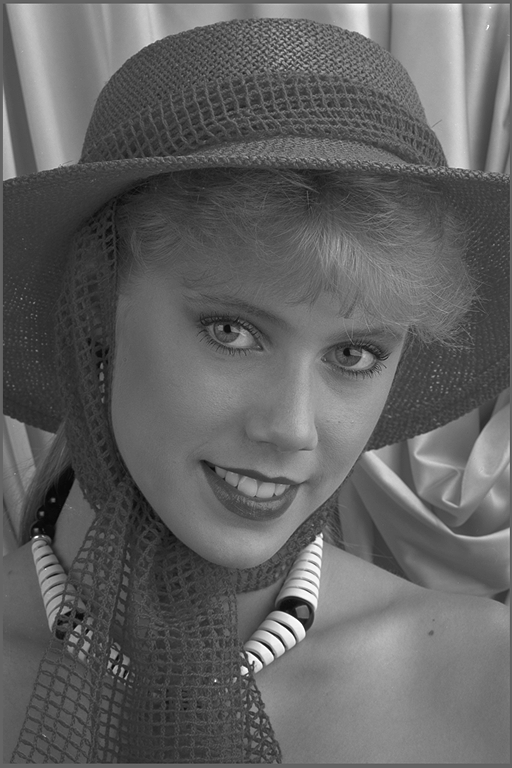
\includegraphics[width=0.9\textwidth]{img03y.png}
					\caption{Original img03y.tif}
				\end{subfigure}
				\begin{subfigure}{0.3\textwidth}
					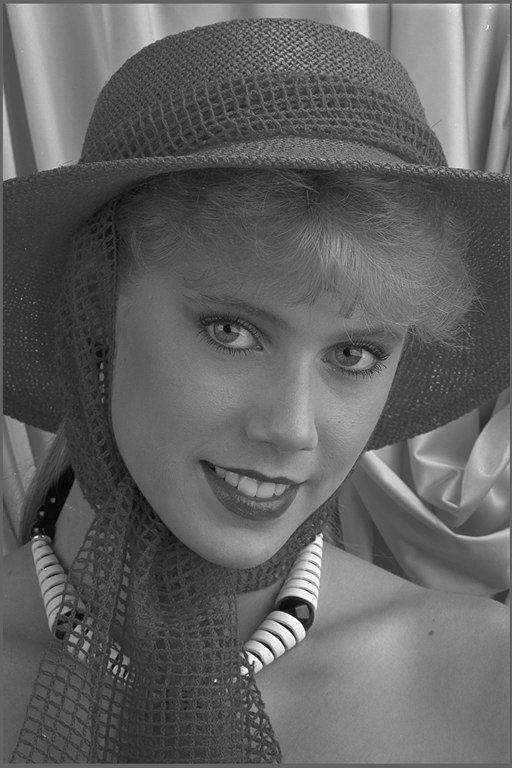
\includegraphics[width=0.9\textwidth]{img03y_1.png}
					\caption{Restored Image}
				\end{subfigure}
				\begin{subfigure}{0.3\textwidth}
					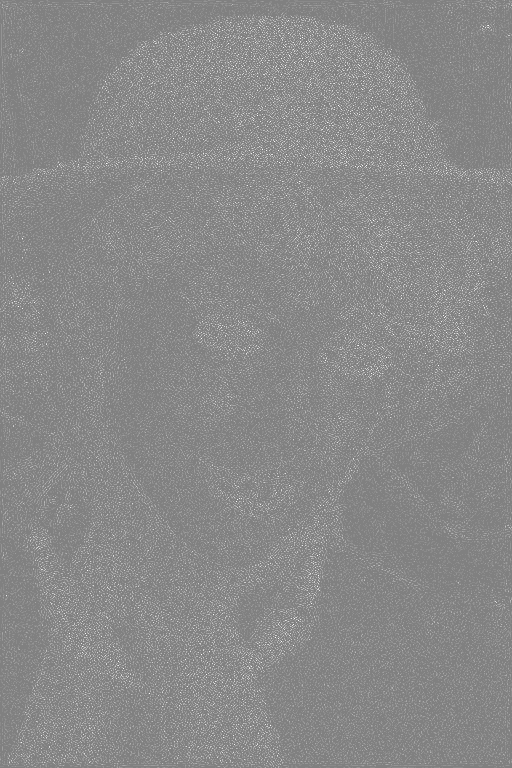
\includegraphics[width=0.9\textwidth]{img03y_diff_1.png}
					\caption{Diff Image}
				\end{subfigure}
				\caption{Original vs. Restored vs. Difference Images, $\gamma$=0.25}
			\end{figure}
			\begin{figure}[!htb]
				\begin{subfigure}{0.3\textwidth}
					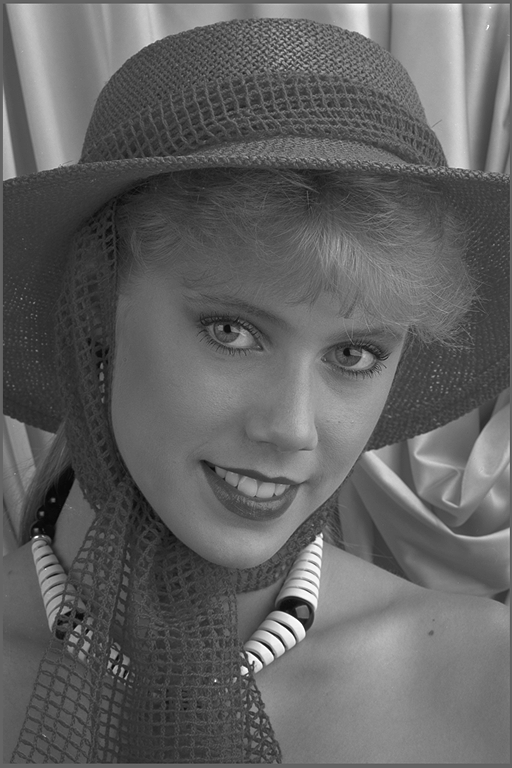
\includegraphics[width=0.9\textwidth]{img03y.png}
					\caption{Original img03y.tif}
				\end{subfigure}
				\begin{subfigure}{0.3\textwidth}
					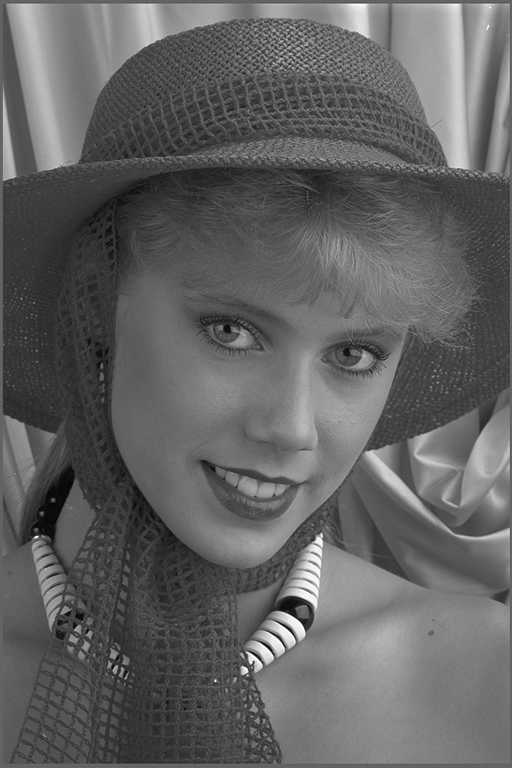
\includegraphics[width=0.9\textwidth]{img03y_2.png}
					\caption{Restored Image}
				\end{subfigure}
				\begin{subfigure}{0.3\textwidth}
					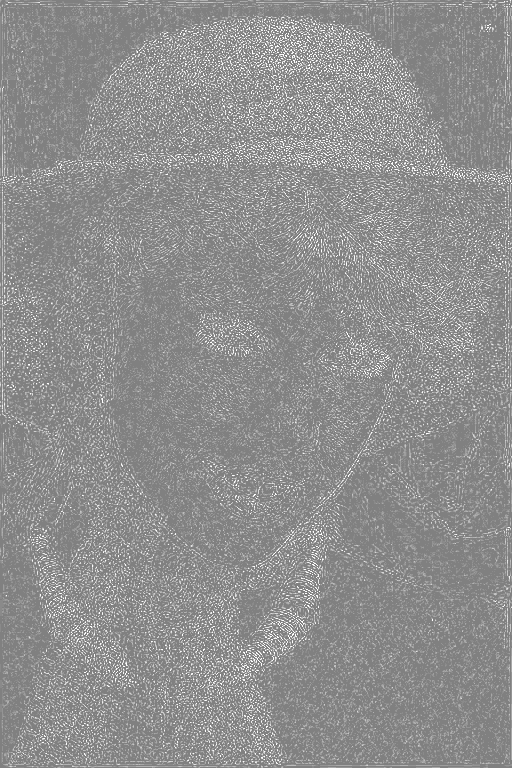
\includegraphics[width=0.9\textwidth]{img03y_diff_2.png}
					\caption{Diff Image}
				\end{subfigure}
				\caption{Original vs. Restored vs. Difference Images, $\gamma$=1}
			\end{figure}
			\begin{figure}[!htb]
				\begin{subfigure}{0.3\textwidth}
					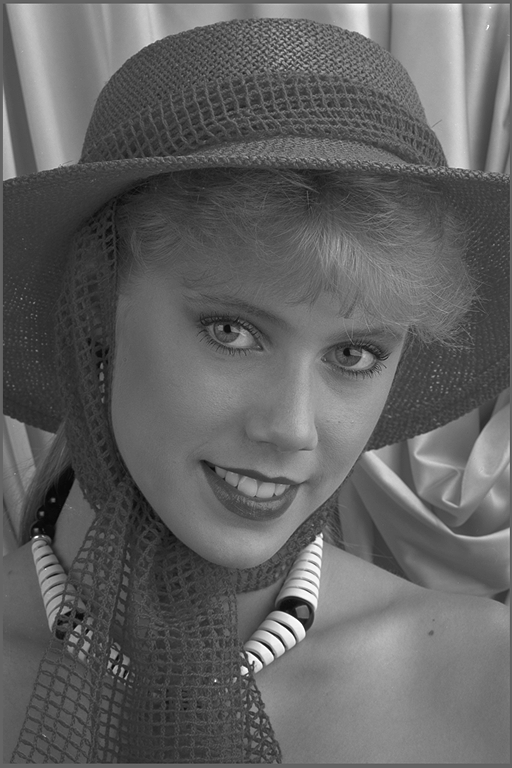
\includegraphics[width=0.9\textwidth]{img03y.png}
					\caption{Original img03y.tif}
				\end{subfigure}
				\begin{subfigure}{0.3\textwidth}
					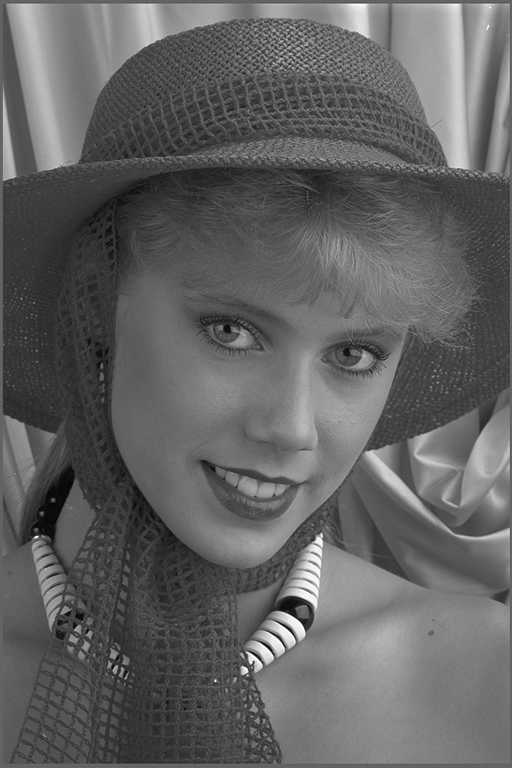
\includegraphics[width=0.9\textwidth]{img03y_2.png}
					\caption{Restored Image}
				\end{subfigure}
				\begin{subfigure}{0.3\textwidth}
					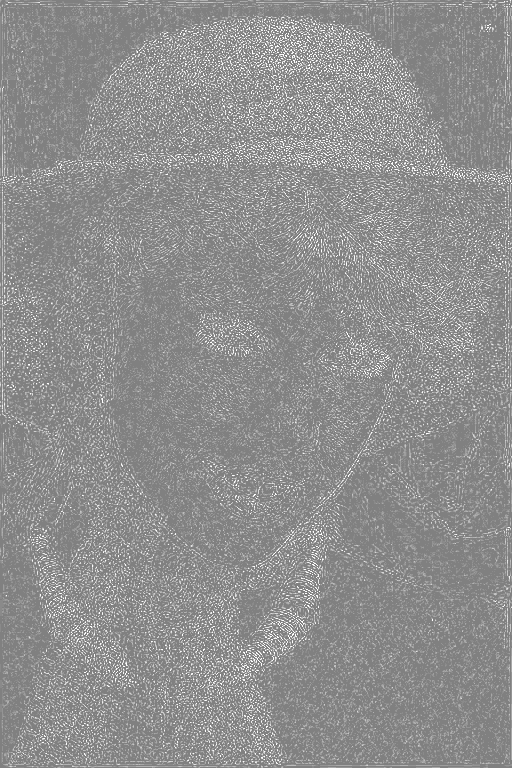
\includegraphics[width=0.9\textwidth]{img03y_diff_2.png}
					\caption{Diff Image}
				\end{subfigure}
				\caption{Original vs. Restored vs. Difference Images, $\gamma$=4}
			\end{figure}
			\\
			\\
			\\
			\\
			\\
			\\
			\\
			\\
	\subsection{Differential Encoding and the Zig-Zag Scan Pattern}
		Nothing due for report.
	\subsection{Exercises}
		\subsubsection{Image Formed By the DC Coefficients}
			The image below is formed by the DC components of the original image; it
			looks similar to the original image but the resolution is lowered since
			it is an window-average of the original image. \\
			\begin{figure}[!htb]
				\begin{center}
					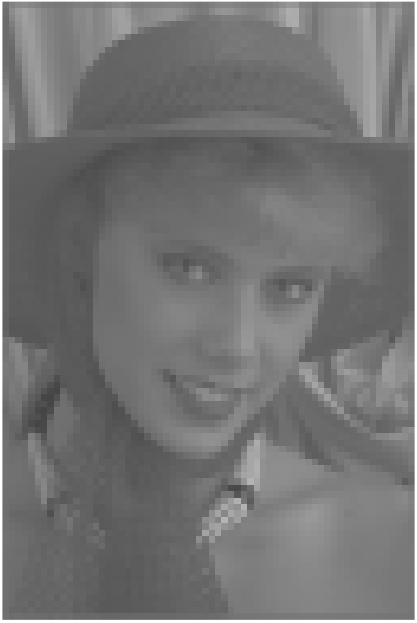
\includegraphics[width=0.3\textwidth]{img03y_dcc.png}
					\caption{DC Coefficients Image}
				\end{center}
			\end{figure}
		\subsubsection{Explanation}
			The DC coefficients of adjacent blocks are correlated because the average
			intensity of neighboring pixels is usually close in terms of values for a
			natural image.
		\subsubsection{Plot of Mean Value of AC Coefficients for $\gamma$=1.0}
			\begin{figure}[!htb]
				\begin{center}
					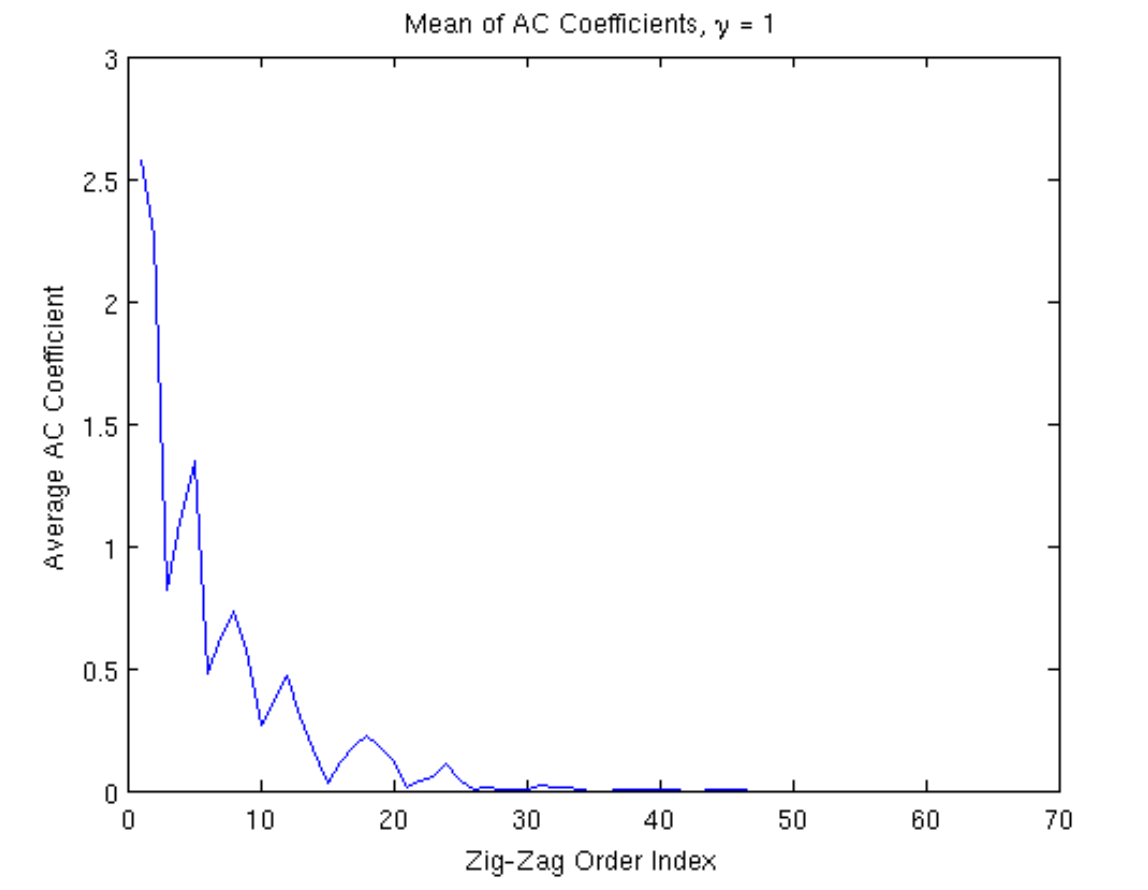
\includegraphics[width=0.6\textwidth]{mean_zigzag.png}
					\caption{Average DCT AC Value}
				\end{center}
			\end{figure}

%----------------------------------------------------------------------------------------
%	SECTION 3
%----------------------------------------------------------------------------------------

\section{Entropy Encoding of Coefficients}
	\subsection{C Code for Subroutines}
		\subsubsection{JPEGdef.c}
			\inputminted[tabsize=2]{c}{../source/jpeg/JPEGdefs.c}
	\subsection{C Code for Main Program}
		\subsubsection{JPEGencode.c}
			\inputminted[tabsize=2]{c}{../source/jpeg/JPEG_encode.c}
	\subsection{Email the Encoded Image}
		The encoded image was submitted.
	\subsection{Three Plots from xv}

\end{document}
